\lez{22}{08-04-2020}{}
\subsection{Estensione dinamica: funzione di Van Hove.}
\label{subsec:Estensione dinamica}
L'espansione dinamica della funzione di correlazione di coppia $g(r)$ è chiamata $G(r,t)$ definita come:
\[\begin{aligned}
	G(r,t) 
	=&
	\frac{1}{N}\sum_{i,j}^{} \left<\delta(r-(r_i(0)-r_j(0))) \right>=\\
	=&
	\frac{1}{\rho }\left<\rho (0,0)\rho (r,t) \right>
.\end{aligned}\]
Dove abbiamo rimosso la media temporale dalla definizione di $\rho $, in questo modo ricompare la sua dipendenza dal tempo.\\
In generale per i sistemi non isotropi si ha anche che:
\[
	G(r,t) = \frac{1}{N}\int d\v{r}'\rho (\v{r}',0)\rho (\v{r}'+\v{r},t)
.\] 
Come per la $g(r)$ è possibile dividere questa funzione in una parte "self" ed una riguardante particelle differenti:
\[
	G(r,t) = G_s(r,t) + G_d(r,t)
.\] 
Notiamo che per $t=0$ si ha:
\[
	G(r,t=0)=\delta(r)+\rho g(r)
.\] 
Quindi nel limite statico torna lo screenshot del sistema con tutta l'analisi della scorsa lezione. L'utilità di introdurre una $G(r,t)$ è che dalle sole $S(k)$ e $g(r)$ non è possibile distinguere un sistema amorfo da uno liquido.\\
Su scale temporali grandi nei liquidi possiamo assumere che la correlazione temporale tra le particelle vada perduta: la media statistica del prodotto delle due densità è il prodotto delle medie statistiche.
\[
	G(r,t) \approx \frac{1}{N}\int d\v{r}'' \rho (\v{r}-\v{r}'')\rho (\v{r}'')
.\] 
Questo implica che nei liquidi che $G(r,\infty)\sim G_d(r,\infty) \to \rho$ mentre $G_s(r,\infty)\to \frac{1}{V} \sim 0$ dove $V$ è il volume medio occupato da una particella (questi andamenti sono dovuti al fatto che il numero di coppie scala come $N^2$ mentre il numero di particelle scala come $N$?). Possiamo vedere l'annullamento della $G_s$ come la perdita della autocorrelazione della particella.\\
Nei solidi viceversa si ha che il volume $V$ in cui una particella è confinata è piccolo, quindi non vi sarà l'annullamento della $G_s$.\\
Notiamo che la perdita di memoria (o correlazione) da parte di un liquido può caratterizzare il liquido: maggiore perdita di correlazione e minore sarà la viscosità del liquido stesso.
\subsubsection{Riassunto sulla $G(r)$}
\label{subsubsec:Riassunto sulla $G(r)$}
\begin{itemize}
	\item La funzione di Van Hove descrive la correlazione spaziale e temporale tra
		le fluttuazioni di densità:
		\[
			G(r,t) = G_s(r,t) + G_d(r,t)
		.\] 
	\item Istante iniziale: 
	\[
		G(r,0) = \delta(r) + \rho g(r)
	.\] 
	\item Dopo un tempo scala molto grande: 
		\begin{itemize}
			\item Liquidi:
			\[
				G(r,\infty) = \frac{1}{N} \int d\v{r}''
				\rho (\v{r}-\v{r}'')\rho (\v{r}'')
				=
				\begin{cases}
					&G_s = \frac{1}{V}\to 0\\
					&G_d = \rho 
				\end{cases}
			.\] 
			\item Cristalli:
			\[
				G(r,\infty)=\frac{1}{N}\int d\v{r}'' 
				\rho (\v{r}-\v{r}'')\rho (\v{r}'') 
				=
				\begin{cases}
					&G_s \sim \rho _\text{loc} (r)\\
					&G_d \xrightarrow{FT}\left| \rho (k) \right| ^2
				\end{cases}
			.\] 
		\end{itemize}
\end{itemize}
\subsubsection{Funzione di scattering intermediata.}
\label{subsubsec:Fonzione di }
La trasformata (spaziale) di Fourier della funzione di Van Hove è chiamata la funzione di scattering intermediata:
\[\begin{aligned}
	F(k,t) 
	=&
	\int d\v{r}e^{i\v{k}\cdot\v{r}}G(r,t) =\\
	=&
	\frac{1}{\rho }\int d(\v{r}-\v{r}')e^{i\v{k}\cdot\left( \v{r}-\v{r}' \right) }
	\left<\rho (\v{r}',0)\rho (r,t) \right> =\\
	=&
	\frac{1}{N}\left<\overline{\rho}(-k,0)\overline{\rho}(k,t)\right>
.\end{aligned}\]
Questa funzione misura la correlazione temporale delle fluttuazioni della densità ad un dato numero d'onda $\v{k}$. Può esser vista come la probabilità che la fluttuazione di densità avente vettore d'onda $\v{k}$ generata al tempo 0 sia ancora presente dopo un tempo $t$.\\
Proprio come la funzione $G$ anche la sua trasformata può essere separata nella parte self e nella parte a diverse particelle:
\[\begin{aligned}
	F(\v{k},t) 
	=&
	F_s(\v{k},t) + F_d(\v{k},t) =\\
	=&
	\frac{1}{N}
	\left<\sum_{i}^{} \exp(i\v{k}\left( \v{r}_i(t)-\v{r}_i(0)\right) ) \right>
	+ \frac{1}{N}
	\left<\sum_{i\neq j}^{} \exp(i\v{k}\left( \v{r}_i(t)-\v{r}_j(0) \right) ) \right>
.\end{aligned}\]
\begin{figure}[ht]
	\centering
	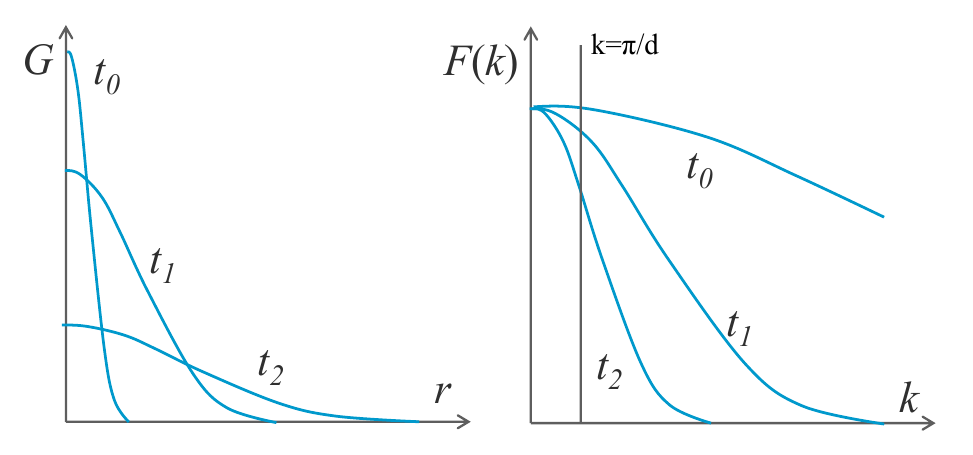
\includegraphics[width=0.6\textwidth]{figures/Gs-Fs.png}
	\caption{Andamento della funzione $G_s$ confrontato con la $F_s$ al variare del tempo.}
	\label{fig:figures-Gs-Fs-png}
\end{figure}
Dalla Figura~\ref{fig:figures-Gs-Fs-png} possiamo notare che la $F(k)$ misura il decadimento temporale della autocorrelazioni temporali del sistema. Quindi ci dice quanta memori ha il sistema della dinamica delle singole particelle.\\
Per misurare la $F$ solitamente si sonda con lunghezze d'onda dell'ordine di $\pi/d$ con $d$ distanza media tra le particelle e può dirci se un materiale si trova nello stato solido o nello stato liquido. 
\begin{figure}[ht]
	\centering
	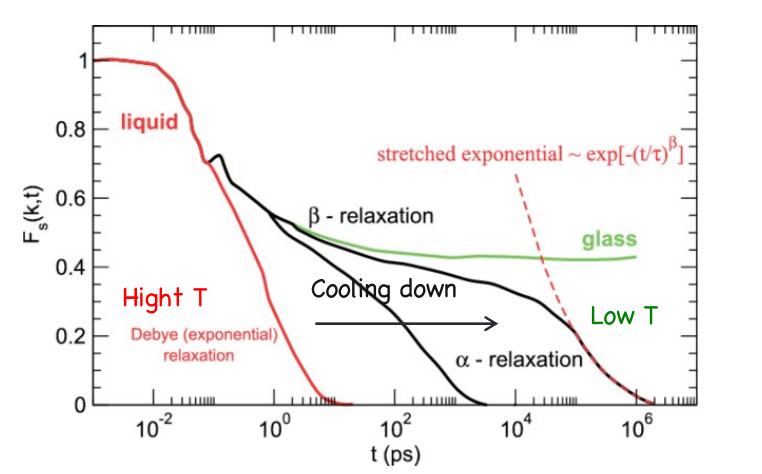
\includegraphics[width=0.34\textwidth]{figures/Fsolido-liquido.png}
	\caption{Osservazione dello stato della materia tramite $F(k)$.}
	\label{fig:figures-Fsolido-liquido-png}
\end{figure}
In Figura~\ref{fig:figures-Fsolido-liquido-png} possiamo notare i diversi andamenti di $F(k)$ al variare del tempo in scala logaritmica.\\
La parte in alto nel grafico piatta indica il tempo in cui la particella preserva la sua autocorrelazione poiché non ha ancora iniziato ad urtare con le altre (questa zona è detta balistica costante).\\
Aumentando la temperatura nel liquido avviene un veloce decadimento detta fase di Debye, questo è un processo collegato alla viscosità del liquido.\\
Abbassando la temperatura questo andamento di caduta diventa sempre più lento, il meccanismo di perdita di correlazione diventa sempre meno efficiente fino a che a temperature molto basse non si stabilizza come nel caso del vetro.\\
Anche nei cristalli possiamo avere dei processi di rilassamento dovuti ai fononi, in approssimazione armonica questi non interagiscono tra loro mentre aggiungendo un termine di interazione possono interagire e far perdere correlazione temporale tramite un decadimento delle oscillazioni.
\subsection{"Fononi" e fattore di struttura dinamico.}
\label{subsec:Collegamento tra la funzione di scattering intermedia ed i fononi}
Essendo la densità la media della posizione delle particelle la fluttuazione della densità deve essere legata alla variazione della posizione delle particelle.\\
Di conseguenza la $\overline{\rho }(k,t)$ descrive la variazione temporale delle fluttuazioni di densità "wavelike" con una data lunghezza d'onda corrispondente appunto ad un fonone nel cristallo.\\
Le vibrazioni collettive coerenti di fluttuazioni di densità in un fluido sono la generalizzazione dei fononi per i fluidi, $\rho (k,t)$ può essere usata come variabile collettiva dei modi normali. Se tali modi sono presenti ci si aspetta che varino nel tempo con una frequenza del tipo $e^{i\omega _kt}$. In conclusione $F(k,t)$ è collegata a quanto più esiste di simile ai fononi nei liquidi.\\
Con queste basi è possibile calcolare anche la trasformata di Fourier temporale di $F(k,t)$ ed associarla allo spettro delle fluttuazioni di densità, questa quantità è definita fattore di struttura dinamico:
\[\begin{aligned}
	S(k,\omega )
	=&
	\int dt F(k,t) e^{-i\omega t}=\\
	=&
	\int dt \int d\v{r}G(r,t) e^{i\left( \v{k}\cdot\v{r}-\omega t \right)}=\\
	=&
	\frac{1}{N}\int \left<\overline{\rho }(-k,0)\overline{\rho }(k,t) \right>e^{-i\omega t}
.\end{aligned}\]
Per definizione abbiamo che:
\[
	\int\frac{d\omega }{2\pi}S(k,\omega )= F(k,0)=S(k)
.\] 
Che si ottiene usando le definizioni di $S(k,\omega )$ e di $S(k)$. Questa quantità deve quindi essere legata alla $S(k)$: mentre quest'ultima permetteva scambio di momento angolare (quindi $k$) adesso il fattore di struttura dinamico permette anche scambio di energia ($\omega $), quindi permette lo scattering inelastico!\\
Possiamo quindi affermare che il fattore di struttura dinamico è proporzionale alla sezione d'urto di scattering inelastica. \\
Se incidiamo nel liquido con elettroni lo scattering inelastico farà si che tali protoni perdano energia, tale energia viene ceduta ai fononi.
\subsection{Approssimazione per le funzioni di struttura dinamica.}
\label{subsec:Approssimazione per le funzioni di struttura dinamica.}
Abbiamo visto alcune teorie di chiusura per le funzioni statiche, nel caso dinamico è ancora più complicato. \\
Un possibile metodo per risolvere è quello di riscrivere la $F$ come:
\[\begin{aligned}
	F(\v{k},t) 
	=&
	F_s(\v{k},t) + \frac{1}{N}
	\sum_{i\neq j}^{} 
	\left<e^{i\v{k}\left( \v{r}_i(0)-\v{r}_j(0) \right)}
	e^{i \v{k}\left( \v{r}_i(t)-\v{r}_j(0) \right)}\right> =\\
	\approx &
	F_s(\v{k},t) + \frac{1}{N}
	\sum_{i}^{} \left<e^{i\v{k}\left( \v{r}_i(t)-\v{r}_i(0) \right) } \right>
	\left[ \sum_{i}^{} e^{i\v{k}\left( \v{r}_i(0)-\v{r}_j(0) \right) }-1 \right] =\\
	=&
	F_s(\v{k},t)F(\v{k},0)
.\end{aligned}\]
Abbiamo assunto così che la media del prodotto sia il prodotto delle medie. Questa approssimazione è equivalente a separare le correlazioni spaziali e temporali. In questo modo si assume che la parte di correlazione temporale della funzione si comporti in modo indipendente dal resto.\\
In altre parole fissata la parte temporale a $t=0$ si assume che tale parte si propaghi nel tempo come conseguenza del moto della particella stessa, senza nessuna modifica intrinseca. Di conseguenza abbiamo che:
\[
	F(k,t)=S(k,t)F_s(k,t) \quad \quad 
	G(r,t) = G_s(r,t)+\rho 
	\int d\v{r}'g(r')G_s(\left| \v{r}-\v{r}' \right|, t) \quad \quad
	S(k,\omega ) = S(k)S_s(k,\omega )
.\] 
Questa approssimazione porta con se alcuni problemi:
\begin{itemize}
	\item Non funziona bene per tempi lunghi (nel regime idrodinamico).
	\item Non soddisfa la legge di conservazione della quantità di moto.
\end{itemize}
Tuttavia ha il grosso vantaggio di includere in maniera naturale la funzione $S(k)$ e tutte le approssimazioni viste nelle scorse lezioni per questa.\\
\subsection{Collegamento con le funzioni di risposta del fluido}
\label{subsec:Collegamento con le funzioni di risposta del fluido}
Le fluttuazioni possono essere incluse nel fluido come media di un qualche potenziale esterno. Nella teoria di risposta lineare queste sono proporzionali queste sono proporzionali alla funzione di risposta $\chi$:
 \[
	 \delta\rho (r,t)=\int d\v{r}'\int_{-\infty}^{t} 
	 \chi(\v{r}-\v{r}',t-t') v(\v{r}',t,)dt
	 \xrightarrow{\text{limite stazionario}}
	 \delta\rho (\v{r})=\int d\v{r}'\chi_s(\v{r}-\v{r}')v(\v{r}')
.\] 
Dove $\chi_s$ indica la suscettibilità:
\[
	\chi_s(\v{r}-\v{r}') = \int\chi(\v{r}-\v{r}',t-t')dt
.\] 
Entrambe le funzioni ($\chi$ e $S$) si riferiscono ad una risposta nella densità del sistema ad una perturbazione esterna, infatti entrambe possono essere calcolate come media della teoria perturbativa.\\
Il calcolo diretto della funzione di risposta che affronteremo nella lezione seguente porterà alle seguenti relazioni (dal calcolo quantistico alla temperatura nulla):
\[
	\overline{\chi}(\v{k},\omega ) = \overline{\chi}'(\v{k},\omega )
	+ i \overline{\chi}''(\v{k},\omega )
.\] 
Con 
\[
	\overline{\chi}''(\v{k},\omega ) = \frac{\rho }{2\hbar}
	\left[ S(k,\omega )-S(-k,-\omega ) \right] 
.\]
Questa è una forma del \textit{Teorema fluttuazione dissipazione}: la parte immaginaria della funzione di riposta è proporzionale alla energia dissipata quando il sistema risponde ad un piccolo stimolo esterno; il fattore di struttura dinamico descrive allora la correlazione temporale spettrale delle fluttuazioni all'equilibrio in assenza di stimoli esterni.\\
Quanto detto sopra deriva dalla forma quantistica della funzione di risposta. Usando la distribuzione termica delle fluttuazioni come:
\[
	\overline{\chi}''(\v{k}, \omega ) = \frac{\rho }{2\hbar}S(k,\omega )
	\left[ 1- e^{-\hbar\omega /kT}  \right] 
	\xrightarrow{\text{Limite classico}}
	\overline{\chi}''(\v{k},\omega ) = \frac{\rho \omega }{2kT} 
	\propto \left<\left| \rho _k(\omega ) \right| ^2 \right>
.\]
Il principio di causalità implica che la funzione di riposta deve soddisfare qualche relazione esatta di somma (?) e che le parti reale/immaginaria di tale funzione devono essere collegate dalle relazioni di KK, quindi:
\[
	\overline{\chi}'(\v{k},\omega ) 
	= \frac{1}{\pi}\int d\omega' 
	\frac{\overline{\chi}''(\v{k},\omega )}{\omega '-\omega -i\eta}
	\implies
	S(k) = \frac{kT}{\rho }\overline{\chi}(\v{k},0)
.\] 
Dove adesso riconosciamo la relazione di Ornstein Zernike generalizzata: in questa forma la $\overline{\chi}(\v{k},0)$ rappresenta la compressibilità isoterma del sistema.
